Find the transfer function from force input $f$ to position output $x$ for the system below
\begin{center}
\begin{tikzpicture}[scale=1.75,inner sep=0pt,outer sep=0pt,very thick]
\draw (4.7,0) node (a) {}; 
 
\draw (0,0) node (gnd1) {\input{\mainfolder/DrawingElements/MechanicalElements/ground.tex}};
\draw (1,.3) node (K1) {\begin{tikzpicture}
\draw (.75,0) node[inner sep=0,outer sep=0] (K1) {\begin{tikzpicture}
\draw (.75,0) node[inner sep=0,outer sep=0] (K1) {\begin{tikzpicture}
\draw (.75,0) node[inner sep=0,outer sep=0] (K1) {\input{\mainfolder/DrawingElements/MechanicalElements/spring.tex}};
\draw (K1)  node[above=6pt] {$k$};
\draw[very thick] (K1.180) -- ++(-.2,0);
\draw[very thick] (K1.0) -- ++(0.2,0);
\draw[<-,thick] (K1.0) ++(.2,0) -- ++(.5,0) node[right] {$f$};
\draw[<-,thick] (K1.180) ++(-.2,0) -- ++(-.5,0) node[left] {$f$};
\draw[|->,thick] (K1.180) ++(-.2,.4) node[above=2pt] {$x_{1}$} -- ++(.5,0);  
\draw[|->,thick] (K1.0) ++(.2,.4) node[above=2pt] {$x_{2}$} -- ++(.5,0);  
\draw<2-> (K1) ++(0,-.6) node {$f=k(x_{1}-x_{2})$};
\end{tikzpicture}
};
\draw (K1)  node[above=6pt] {$k$};
\draw[very thick] (K1.180) -- ++(-.2,0);
\draw[very thick] (K1.0) -- ++(0.2,0);
\draw[<-,thick] (K1.0) ++(.2,0) -- ++(.5,0) node[right] {$f$};
\draw[<-,thick] (K1.180) ++(-.2,0) -- ++(-.5,0) node[left] {$f$};
\draw[|->,thick] (K1.180) ++(-.2,.4) node[above=2pt] {$x_{1}$} -- ++(.5,0);  
\draw[|->,thick] (K1.0) ++(.2,.4) node[above=2pt] {$x_{2}$} -- ++(.5,0);  
\draw<2-> (K1) ++(0,-.6) node {$f=k(x_{1}-x_{2})$};
\end{tikzpicture}
};
\draw (K1)  node[above=6pt] {$k$};
\draw[very thick] (K1.180) -- ++(-.2,0);
\draw[very thick] (K1.0) -- ++(0.2,0);
\draw[<-,thick] (K1.0) ++(.2,0) -- ++(.5,0) node[right] {$f$};
\draw[<-,thick] (K1.180) ++(-.2,0) -- ++(-.5,0) node[left] {$f$};
\draw[|->,thick] (K1.180) ++(-.2,.4) node[above=2pt] {$x_{1}$} -- ++(.5,0);  
\draw[|->,thick] (K1.0) ++(.2,.4) node[above=2pt] {$x_{2}$} -- ++(.5,0);  
\draw<2-> (K1) ++(0,-.6) node {$f=k(x_{1}-x_{2})$};
\end{tikzpicture}
};
\draw (1,.3) node[above=.2in] {$k$};
\draw (2.7,0) node (M1) {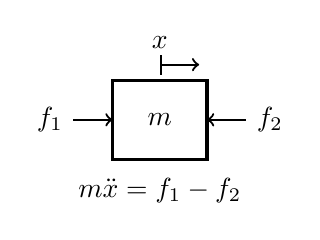
\begin{tikzpicture}
    \draw[very thick] (0,0) rectangle (1.2,1);
    \draw (.6,.5) node {$m$};
    \draw[<-,thick] (1.2,.5) -- ++(.5,0) node[right] {$f_{2}$};
    \draw[<-,thick] (0,.5) -- ++(-.5,0) node[left] {$f_{1}$};
    \draw[|->,thick] (.6,1.2) node[above=2pt] {$x$} -- ++(.5,0);  
        \draw<2-> (.6,-.4) node {$m\ddot{x}=f_{1}-f_{2}$};

\end{tikzpicture}
};
\draw (2.7,0) node {$m$};
\draw[|->] (2.5,.8) node[above=.15in] {$x$} -- ++(.5,0);
\draw (1,-.3) node (D) {\begin{tikzpicture}
\draw[very thick] (-.2,0) -- (0,0);
\draw (.75,0) node {\begin{tikzpicture}
\draw[very thick] (-.2,0) -- (0,0);
\draw (.75,0) node {\begin{tikzpicture}
\draw[very thick] (-.2,0) -- (0,0);
\draw (.75,0) node {\input{\mainfolder/DrawingElements/MechanicalElements/damper.tex}};
\draw (.75,0) node[above=9pt] {$b$};
\draw[very thick] (1.5,0) -- ++(.2,0);
    \draw[<-,thick] (1.5,0) ++(.2,0) -- ++(.5,0) node[right] {$f$};
    \draw[<-,thick] (-.2,0) -- ++(-.5,0) node[left] {$f$};
    \draw[|->,thick] (-.2,.4) node[above=2pt] {$x_{1}$} -- ++(.5,0);  
    \draw[|->,thick] (1.7,.4) node[above=2pt] {$x_{2}$} -- ++(.5,0);  
    \draw (.6,-.6) node {$x=x_{1}-x_{2}$};
  %  \draw (.6,-1.2) node {$f=b\dot{x}$};
\end{tikzpicture}};
\draw (.75,0) node[above=9pt] {$b$};
\draw[very thick] (1.5,0) -- ++(.2,0);
    \draw[<-,thick] (1.5,0) ++(.2,0) -- ++(.5,0) node[right] {$f$};
    \draw[<-,thick] (-.2,0) -- ++(-.5,0) node[left] {$f$};
    \draw[|->,thick] (-.2,.4) node[above=2pt] {$x_{1}$} -- ++(.5,0);  
    \draw[|->,thick] (1.7,.4) node[above=2pt] {$x_{2}$} -- ++(.5,0);  
    \draw (.6,-.6) node {$x=x_{1}-x_{2}$};
  %  \draw (.6,-1.2) node {$f=b\dot{x}$};
\end{tikzpicture}};
\draw (.75,0) node[above=9pt] {$b$};
\draw[very thick] (1.5,0) -- ++(.2,0);
    \draw[<-,thick] (1.5,0) ++(.2,0) -- ++(.5,0) node[right] {$f$};
    \draw[<-,thick] (-.2,0) -- ++(-.5,0) node[left] {$f$};
    \draw[|->,thick] (-.2,.4) node[above=2pt] {$x_{1}$} -- ++(.5,0);  
    \draw[|->,thick] (1.7,.4) node[above=2pt] {$x_{2}$} -- ++(.5,0);  
    \draw (.6,-.6) node {$x=x_{1}-x_{2}$};
  %  \draw (.6,-1.2) node {$f=b\dot{x}$};
\end{tikzpicture}};
\draw (1,-.3) node[below=.22in] {$b$};

\draw (gnd1.0) ++(0,.3) -- (K1);
\draw (gnd1.0) ++(0,-.3) -- (D);
\draw (K1.0) -| (M1.180);
\draw (D.0) -| (M1.180);
\draw[->] (M1) -- ++(1,0) node[right] {$f$};
\end{tikzpicture}
\end{center}
when $m=2$ kg, $b=6$ Ns/m, $k=18$ N/m. Using the linear approximation rules, sketch the Bode plot for this system. For full credit all axes must be labeled and scaled.
\begin{center}
\includegraphics[width=4in]{\mainfolder/LectureNotes/\lecturefolder/HomeworkProblems/blankbode}
\end{center}
